\documentclass[12pt,letterpaper,oneside]{book}

\usepackage{../afitStyleFiles/afitThesis}
\usepackage{../afitStyleFiles/sf298}
\graphicspath{{../Figures/}}

%% Customize your document with your personal information
%% First, comment out the appropriate document type
\afitthesis %%default
% \afitreport
% \dissertation
% \prospectus

\author{Lauren M. Bramblett}
\rank{2nd Lt, USAF}  % If a civilian, comment out this line. 

\docdesignator{AFIT-ENS-MS-19-M-XXX}
\department{Department of Operational Sciences}
\graduationdate{March 21, 2019}

\flytitle{Turbojet Range, Loiter, and Altitude Tradeoff Estimation in Efficient Modeling and Optimization Formulations} 
\title{\MakeUppercase{AFIT/ENS Thesis Primer:}\\
       \MakeUppercase{ a document in \LaTeX}}
                             % Note, if you use \MakeUppercase to put
                             % the title in all uppercase as the style
                             % guide demands, understand that the
                             % command does not allow page breaks ``\\'' 
                             % within its brackets.
\previousdegrees{B.S.}
\acdegree{Master of Science in Operations Research}
 
\committee{{Dr. L. E. Champagne\\Chair},
           {Dr. R. R. Hill\\Reader}
}

\address{2950 Hobson Way\\ Air Force Institute of Technology \\
Wright-Patterson AFB, OH 45433}

\distribution{DISTRIBUTION STATEMENT A\\[-10pt]
\MakeUppercase{Approved for Public Release; distribution unlimited.}
} 

\disclaimer{The views expressed in this document are those of the
author and do not reflect the official policy or position of the
United States Air Force, the United States Department of Defense or
the United States Government.  This material is declared a work of the
U.S. Government and is not subject to copyright protection in the
United States.}

% International students may consider using the following disclaimer
% statement: \dislaimer{The views expressed in this document are those
% of the author(s) and do not reflect the official policy or position
% of the United States Air Force, Department of Defense, United States
% Government, the corresponding agencies of any other government,
% NATO, or any other defense organization.}


%% myFigures.tex
% A common file to store all figure definitions
%
% In preparing your thesis, one of the first things you should do is
% organize your figures.  Then, one of the last things you'll do is
% reorder your figures so they display where you want them to in the
% text.  Organizing figure definitions in a common files helps:
%
%   1. Write new figures using earlier examples.
%
%   2.  Isolate code and minimize the risk of introducing bugs in the
%   final editing process.  Trust me, moving around just one line of
%   code is easier.
%
%   3.  Reuse figures in other papers.  <=== the best reason!
%
% Note command names can not include numbers and special characters.
%
% To make the file more searchable, use naming conventions that map
% the graphics filename labSetup.jpg to the command name \figlabSetup to the
% figure label fig:labSetup.
% 

\newcommand{\figMyFirstLaTeX}{\begin{figure}[tbp]
 \begin{center}
    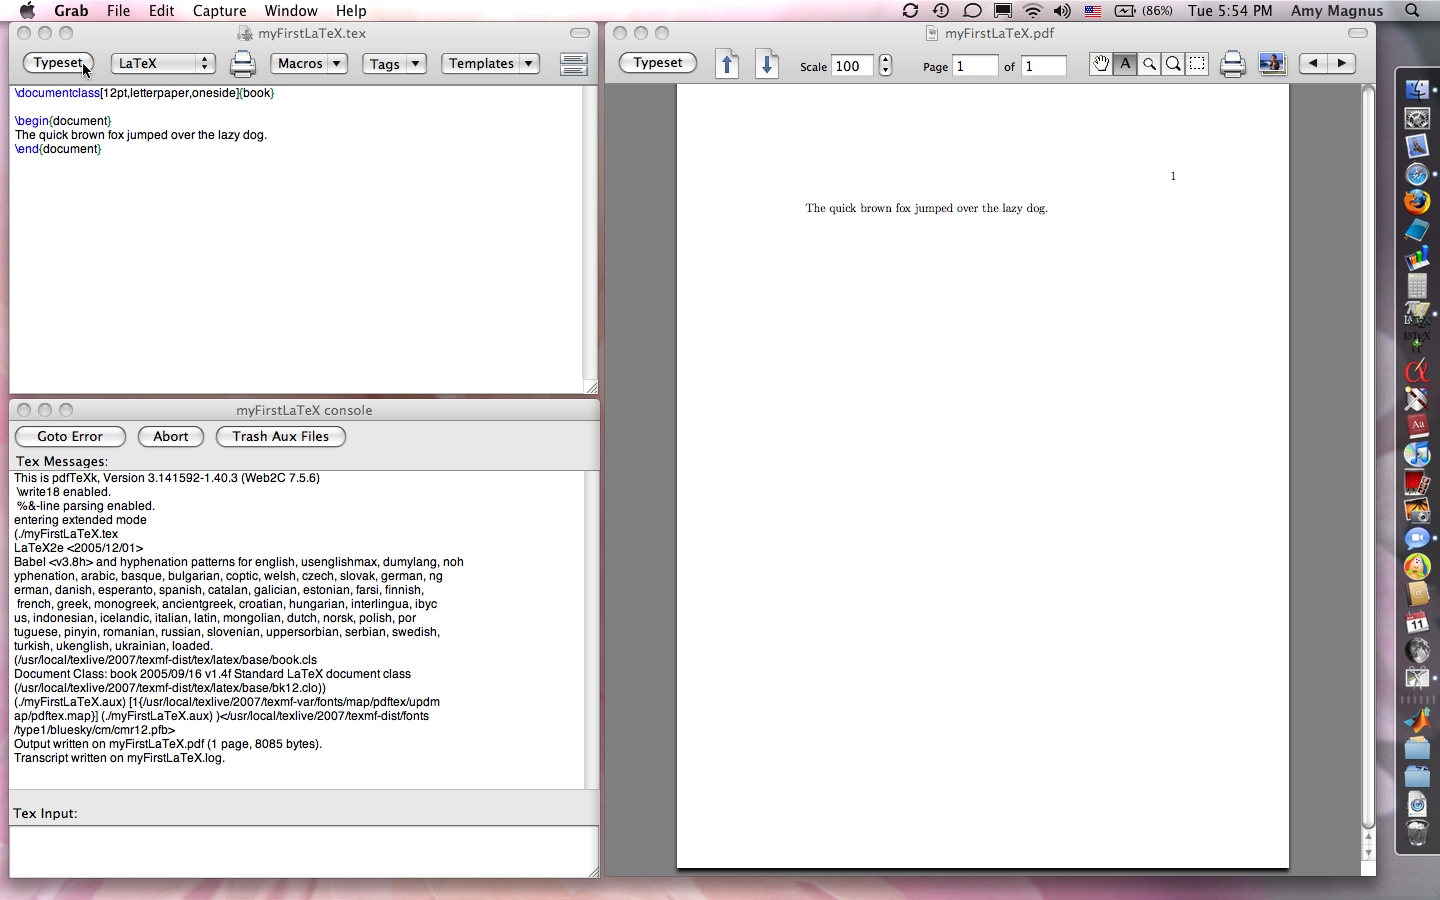
\includegraphics[width=6in]{myFirstLaTeXCursor}
     \caption[\LaTeX\ a very simple document]{Compile a very simple document.}
     \label{fig:MyFirstLaTeX}
 \end{center}
 \vspace{-0.2 in}
\end{figure}
}


\newcommand{\figafitStyle}{\begin{figure}[tbp]
 \begin{center}
    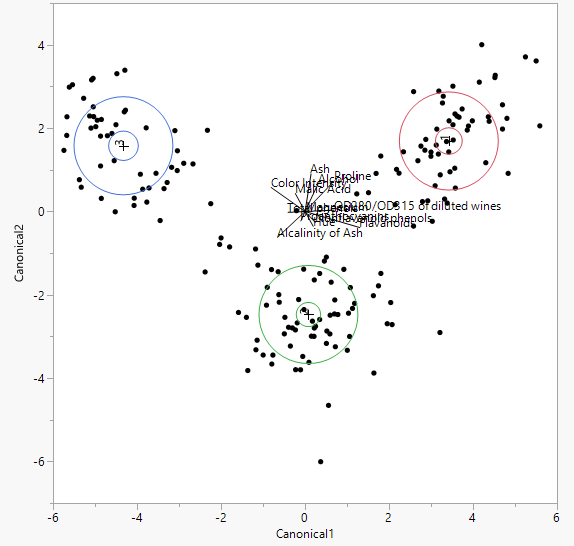
\includegraphics[width=6in]{Thesis/Preamble/Figures/DiscrimAnalysisPlot.PNG}
     \caption{Recompile using afitThesis.sty, the AFIT
     thesis style file.}
     \label{fig:afitStyle}
 \end{center}
\end{figure}
}


\newcommand{\figtitlePage}{\begin{figure}[tbp]
 \begin{center}
    \includegraphics[width=6in]{titlePage}
     \caption{Enter student data in titlePage.tex to customize the
     document's first pages.}
     \label{fig:titlePage}
 \end{center}
\end{figure}
}

\newcommand{\figmyFlypage}{\begin{figure}[tbp]
 \begin{center}
    \includegraphics[width=6in]{myFlypage}
     \caption{Here we have compiled the first four page of a thesis.}
     \label{fig:myFlypage}
 \end{center}
\end{figure}
}

\newcommand{\figmyFirstAbstract}{\begin{figure}[tbp]
 \begin{center}
    \includegraphics[width=6in]{myFirstAbstract}
     \caption{Add an abstract to the front matter of your thesis.}
     \label{fig:myFirstAbstract}
 \end{center}
\end{figure}
}

\newcommand{\figmyFigures}{\begin{figure}[tbp]
 \begin{center}
    \includegraphics[width=5in]{myFigures}
     \caption{Consider defining all your figures in one file.}
     \label{fig:myFigures}
 \end{center}
\end{figure}
}


\newcommand{\figmyFirstFigures}{\begin{figure}[tbp]
 \begin{center}
    \includegraphics[width=6in]{myFirstFigures}
     \caption{Add figures in the main matter of your document; fill in
     the document around your graphics.}
     \label{fig:myFirstFigures}
 \end{center}
\end{figure}
}

\newcommand{\figmyFirstBibTeX}{\begin{figure}[tbp]
 \begin{center}
    \includegraphics[width=6in]{myFirstBibTeX}
     \caption{Add your bibliography.}
     \label{fig:myFirstBibTeX}
 \end{center}
\end{figure}
}




% define custom commands
\newcommand{\regmark}{\raisebox{5pt}{\tiny \circledR}\xspace}
\newcommand{\matlab}{\textsc{Matlab}\regmark}
\newcommand{\trademark}{\raisebox{5pt}{\tiny TM}\xspace}
\newcommand{\mca}{\texttt{Mathematica}\regmark}
\newcommand{\Latex}{\LaTeX\xspace}

% Create a new theorem style called a Corollary.
% If you don't have any, then just comment this out.
%\theoremstyle{plain} % Default
\newtheorem{cor}{Corollary}[chapter]

%Custom Commands for Student

\newcommand{\primerAddress}{{L:$\backslash$Courses$\backslash$PHYS$\backslash$LaTeX}\xspace}


\begin{document}
\frontmatter
	\flyleaf                        
	\disclaimerpage                 
	\titlepageAFIT                      
	\committeepage  
	\begin{abstract}

Writing an abstract here \ldots

\end{abstract}
    

%     As an AFIT graduate student, you are about to write one of the
%     longest documents of your career.  Whether you use a ``what you see
%     is what you get'' (WYSIWYG) interface like Microsoft Word
%     \trademark or a typesetting system like \LaTeX\ldots when you
%     create a digital document, you are writing a program.  The larger
%     any program is, the more bugs it will contain and the more likely
%     the program will result in a catastrophic error.  Common bugs
%     result in improper formating, double words, lost sentences,
%     and---in the worst case---corrupted, unreadable files.
% 
%     Typesetting systems such as \LaTeX\ limit the new lines of code
%     generated with each new document.  As a result, they produce
%     cleaner, easier-to-debug products.  Additional benefits of \LaTeX\
%     are rapid reformatting and high quality typesetting of equations
%     and vector graphics.

	\tableofcontents
	\listoffigures
	\begin{preface}
Welcome to the world of \Latex! Learn \Latex and you can rapidly
produce papers tailored for a wide variety of publications.
When you create a digital
document\ldots whether you use a ``what you see is what you get''
(WYSIWYG) interface like Microsoft Word or a typesetting system like
\Latex\ldots you are writing a program.  In the realm of academic publishing,
\Latex helps us write a better program.   

The best reasons to write with \Latex are high quality equations,
superior graphics, and the automated generation of table of contents,
lists, and bibliographies.  We can create clean 50+ page documents
that reformat in a snap.  Additionally, due to the fact that the
\Latex typesetting system was written by and for academics, many
of its tools are free and run on Microsoft Windows, Mac OS X, and
Linux.

So let's get started.  Download a \Latex distribution for 
your computer platform, set up your editor and compiler and we'll get 
cracking.  
\end{preface}



\mainmatter
	
	\chapter{The First Steps}
		\input{chapter01/mySetup}
		
		\figMyFirstLaTeX
		\section{\Latex a simple document}
		\input{chapter01/startSimple}
		\figafitStyle

		\section{Add a style file}
		\input{chapter01/addStyle}
		
		\figtitlePage
		\section{Add the front matter}
		\input{chapter01/addFrontMatter}

		\figmyFlypage
		\input{chapter01/addAbstract}
		\figmyFirstAbstract
		\input{chapter01/addMoreFrontMatter}

		\section{Add figures to the main matter and start writing}
		\figmyFigures
		\input{chapter01/addFirstResults}
				\figmyFirstFigures
		\input{chapter01/addMainMatter}
		
	\chapter{Customized Environments}
		\input{chapter02/intro}
		\section{Customized lists}
		\input{chapter02/lists}
		\section{Customized environments}
		\input{chapter02/environments}
		\section{Summary}
		\input{chapter02/conclusion}
	\chapter{Conclusion}
	         This primer is intended to give a masters or PhD student the basics of preparing a \Latex document according to the AFIT style guide\cite{AFITStyle}.  If you have further questions on this topic, please contact the author (Dr Amy Magnus x4555) or the office the Dean of Research for more information. \cite{dumBook,dumArticle}
	         
\backmatter
	\singlespace
	\bibliographystyle{authoryear}
	\bibliography{Back/myReferences} 
	\clearpage

   \date{March 2019}
\ReportDate{21--03--2019} \ReportType{Master's Thesis}
\DatesCovered{Jun 2018 --- Mar 2019}

\Title{\centering \MakeUppercase{AFIT/ENP Thesis Primer:}\\
                  \MakeUppercase{ a document in \LaTeX}}

%\Title{\centering \MakeUppercase{Evaluation of Interplanetary
%Magnetic Field Tracing Models Using Impulsive SEP's}}

%\ContractNumber{DACA99--99--C--9999}

%\GrantNumber{}
%\ProgramElementNumber{}
%\ProjectNumber{09ENP???}
%\TaskNumber{}
%\WorkUnitNumber{}

\Author{Lauren M. Bramblett}

\PerformingOrg{Air Force Institute of Technology\\[-1pt]
    Graduate School of Engineering and Management (AFIT/EN)\\[-1pt]
    2950 Hobson Way\\[-1pt]
    WPAFB OH 45433-7765}

\POReportNumber{AFIT--ENS--}

\SponsoringAgency{National Air and Space Intelligence Center\\[-1pt]
1940 Allbrook Drive\\[-1pt]
WPAFB OH 45433-7765\\[-1pt]}
%DSN 271-0690, COMM 937-255-3636\\[-1pt]
%Email: amy.magnus@afit.edu }

\Acronyms{NASIC}
%\SMReportNumber{}
\DistributionStatement{DISTRIBUTION STATEMENT A:\\
\MakeUppercase{Approved for Public Release; distribution unlimited.}}

\Abstract{This primer aids the AFIT student in generating the first draft of
their thesis using \Latex. The primer is produced according the tenets
described within the document.  All source code is provided in a zip
file posted to \primerAddress.  The file structure of this zip file
demonstrates a practical way to organize a thesis with its supporting
materials and---further---illustrates how your document can be produced
with version control.
}

\SubjectTerms{LaTeX,Thesis,typesetting}

\NumberPages{111}
%\ReportClassification{}
%\PageClassification{}
%\AbstractClassification{}
\AbstractLimitation{UU}

\ResponsiblePerson{Dr. L. E. Champagne, AFIT/ENS}

\RPTelephone{(937) 255-3636, x4555; lance.champagne@afit.edu}

\MakeRptDocPage

   \end{document}

